\begin{figure*}[h]                                                           
 
\includegraphics[width=\linewidth]{./media/images/book_candle}%
  \scriptsize{\textsc{\\perhaps not since} written language itself have
    we had a method of challenging our critical thinking skills so impactful for the mind as Interactive Fiction}
  \label{fig:editorial}%                                                 
\end{figure*}                                                                
\begin{quotation} 
\noindent\color{Sepia}{\scriptsize{\textit{\textbf{“In the beginning the Universe was created. This has made a lot of people very angry and been widely regarded as a bad move.” }}}}\\[.5mm]
   \hfill\color{Sepia}{\scriptsize{\textendash Douglass Adams}}
\end{quotation} 
%\begin{abstract}
%\textbf{\emph{“In the beginning the Universe was created. This has made a lot of people very angry and been widely regarded as a bad move.”  \\ \\--- Douglas Adams}}
%\end{abstract}
\newpage
\lettrine[lines=3]{\color{BrickRed}I}{\enspace } stare intently at a small glass computer screen perching over a flat,
rectangular Apple \textsc{ii/c}. The small cathode\textendash ray screen emanates a green
glow from which I read prose presented in all\textendash caps text. From the outside looking in, an
11 year\textendash old boy stares intently at the screen as he sits in his modern 
kneeling chair. His attentive posture and the fingers of both hands rest lightly on the keyboard indicating total concentration. 

From the inside looking out, I see my breath cloud across the face of my brass compass.
\reversemarginpar
\marginpar{
  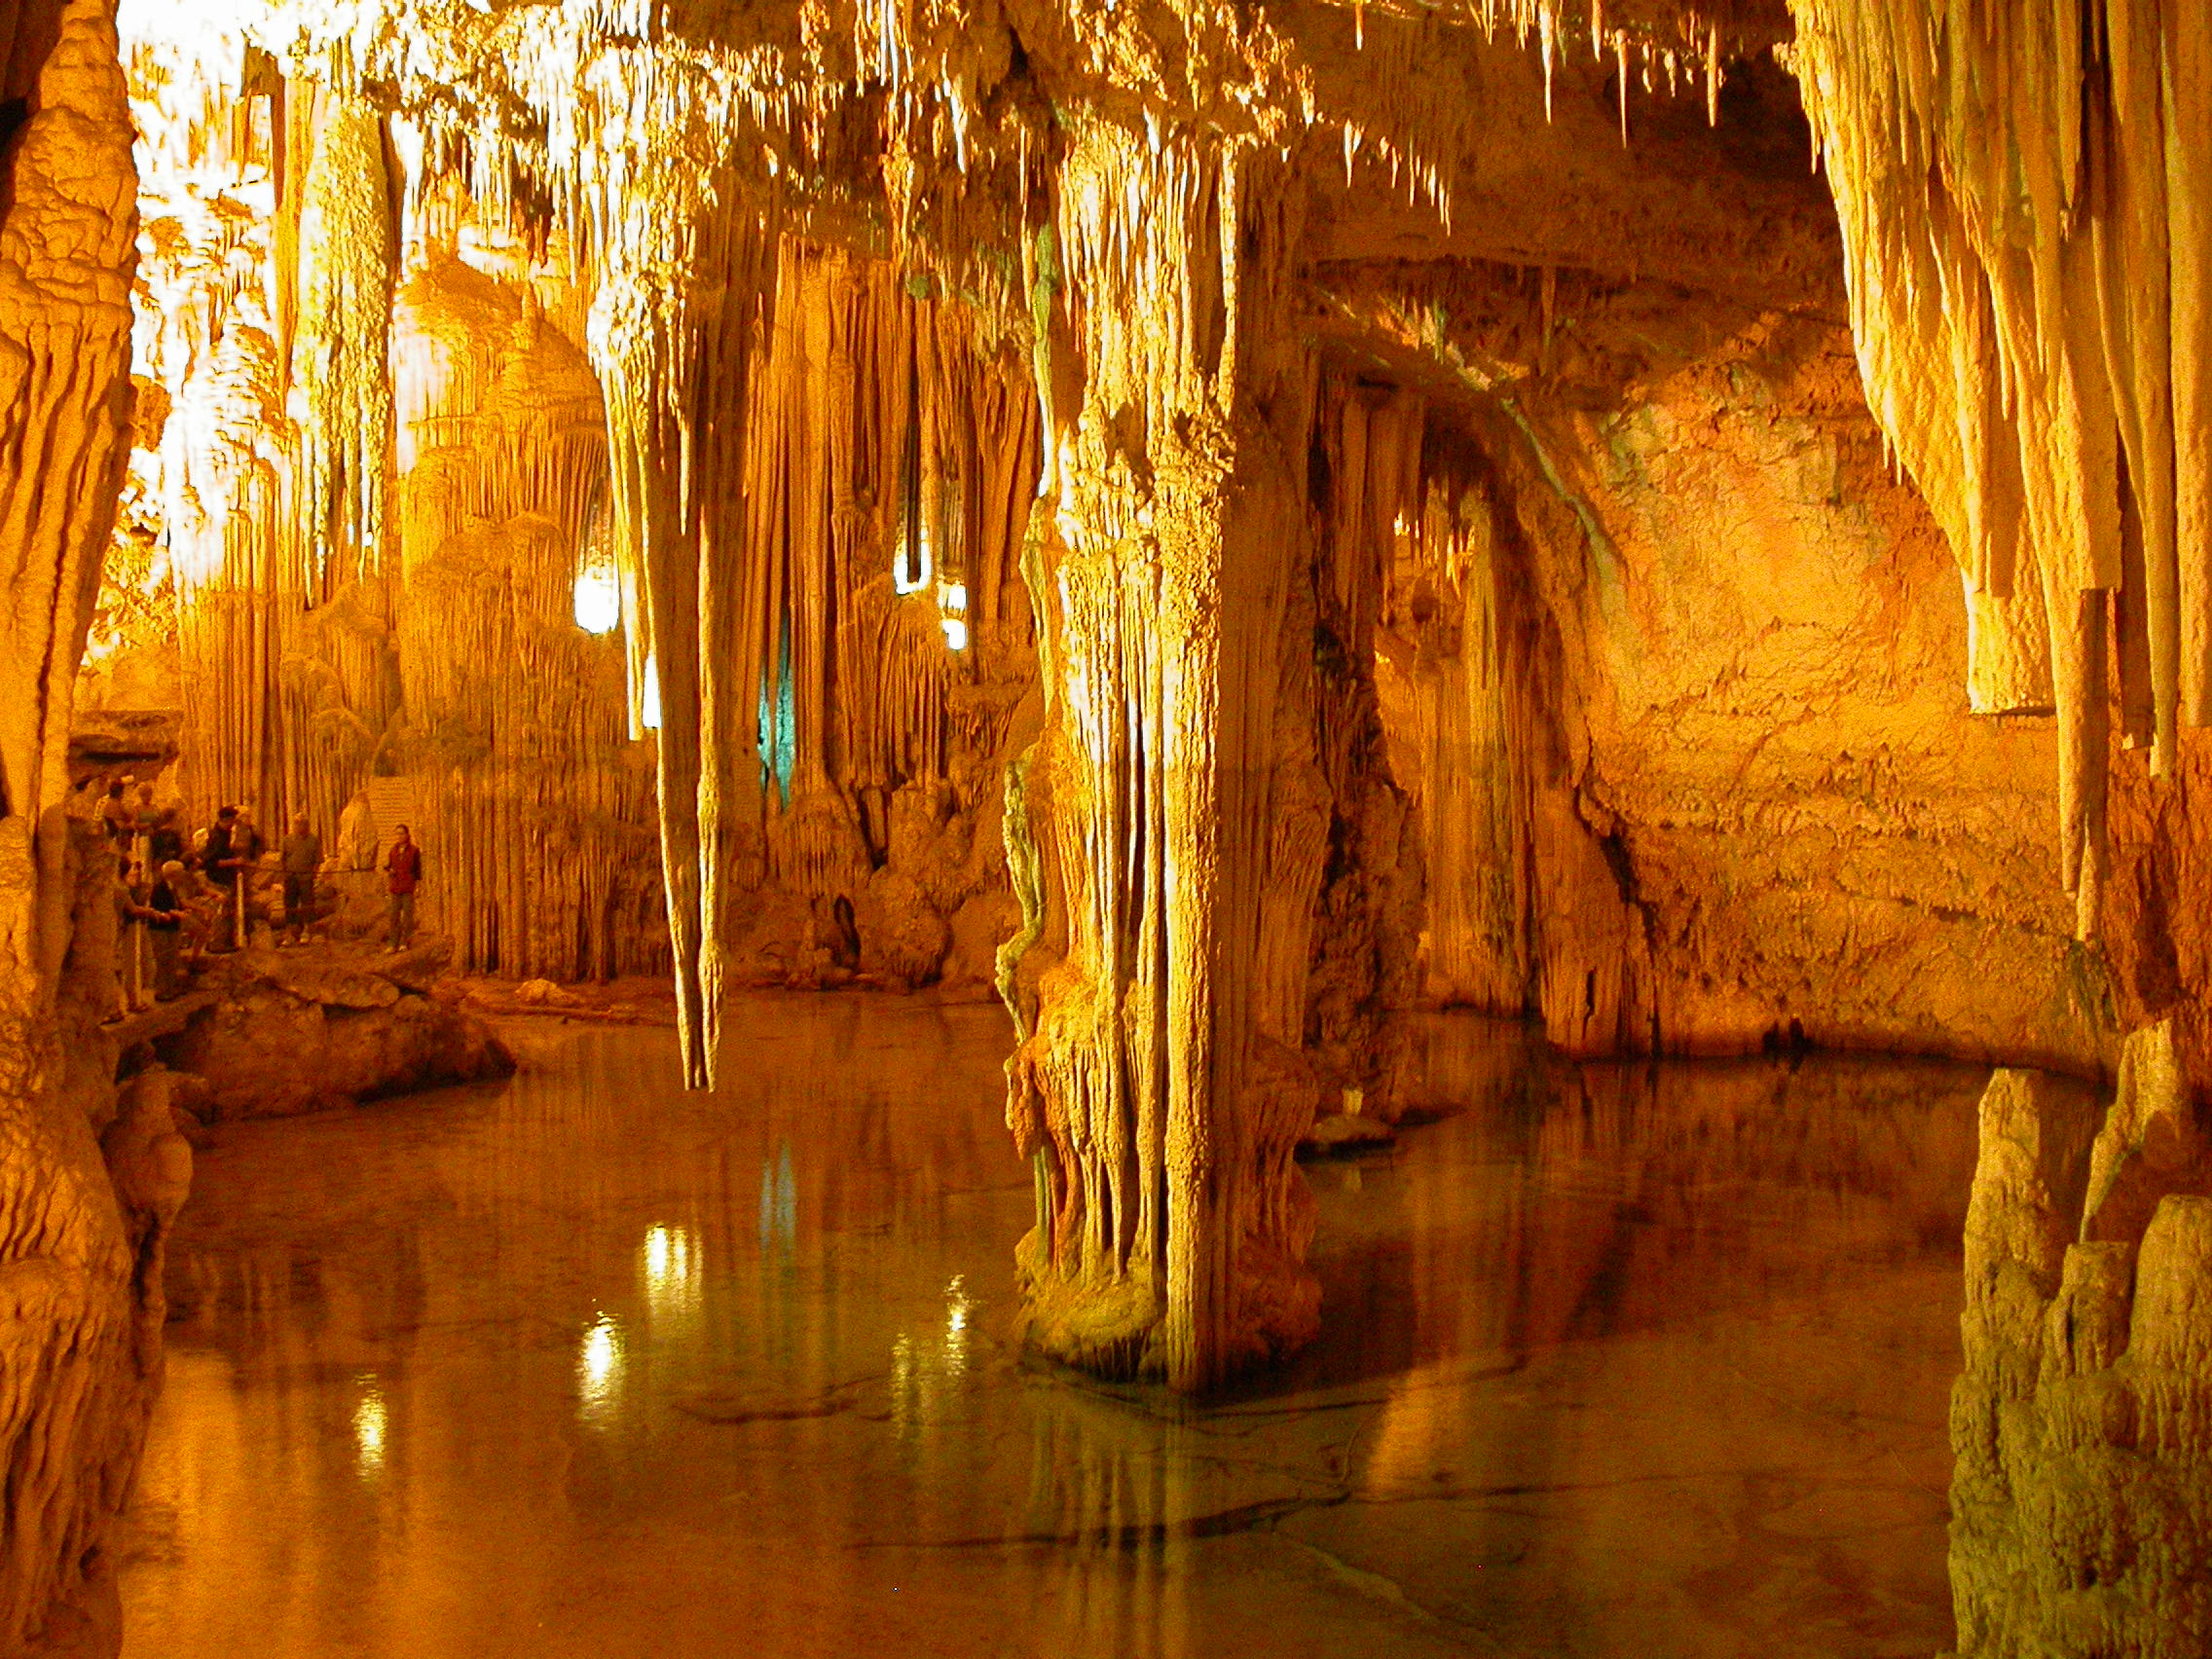
\includegraphics[width=\linewidth]{./media/images/cave}
  \tiny{\textit{Searching every feature for a step to the next challenge. (Photo: {\href{https://commons.wikimedia.org/wiki/File:Grotta_di_nettuno_sardinien.jpg}{\textsc{tobias helfrich}}})}}
  }
I take my bearings by the flickering amber light of the carbide lantern in an
otherwise pitch-black cave.
\marginpar{\vspace{5.75mm}
  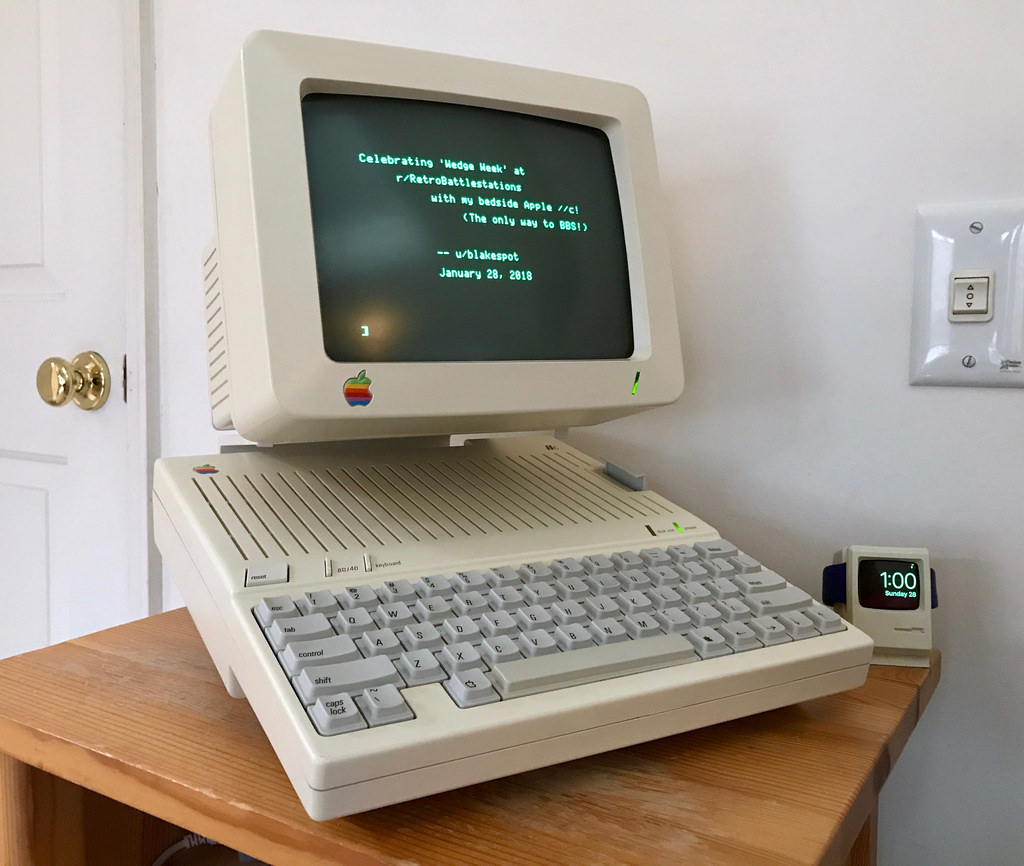
\includegraphics[width=\linewidth]{./media/images/apple}
  \tiny{\textit{The venerable Apple \textit{\textsc{II/c} becomes an Oracle of logic. (Photo:
    \href{https://www.flickr.com/photos/blakespot/}{\textsc{blake peterson})}}}}
}
The lantern's glow encroaches, then recedes, up the cave's walls and over my
shoulder from it's resting place on a cold, wet slab of stone. I clasp shut
my compass and grasp my lantern for a better look around. I hold it higher to
search my surroundings with readied senses. Any detail I can discern from my
surroundings are a welcome receipt that it may further my journey to the crest
of my next discovery. Are there any inscriptions on the cave walls? Do I see
signs of an adjoining passage evidenced by the flow of water? How does this
area fit in with my extended surroundings?

I would be hard\textendash pressed to articulate the concept of logic at this
age; I can only feel it. The game present requires me to think carefully
knowing that only clues from my surroundings and reasoning will advance my 
endeavor. I want badly to know what's around the next corner\textemdash a
passion that drives me to align my thinking to achieve.

\section{the passion never dies}
\label{sec:passion}
Today I write before a high\textendash resolution screen having a dark grey background beneath
multi\textendash colored syntaxed lettering. While the technology advances
greatly from the glowing green \textsc{crt} screens of the past, the foundation
of deduction, logic, and resolute determination have not. The methods the
\normalmarginpar
\marginnote{
  \tiny{\textit{The technology changes but the human drive for knowlege never does}}
}authors teach through play gifts, at least in part, the skills and optimistic
outlook important for a fulfilling life. Don Woods said
\href{https://youtu.be/LRhbcDzbGSU?t=883}{\textsc{in an interview}} that were he
to think about \textsc{if} he would probably not have recognized his work as
a new medium at the time. I humbly submit that he may not also
 have realized that he and Crowther sparked the spirit of sharing and achievement in a new generation by incentivising discovery.

My story is not unique. Hundreds-of-thousands share this experience with some
variation, either by age, place, or both. Legend has it that the venerable text
adventure, \textit{Colossal
  Caves}, shut down all productivity at \textsc{mit}'s computer science
department for a week. Presuming those pioneering souls experienced what I had
playing the game it is not hard to see why: the common thread running through
\textsc{if}'s history are the ways it captures the reader's imagination.

\subsection{active participation}
\label{sec:purpose}
\normalmarginpar
 \marginnote{
  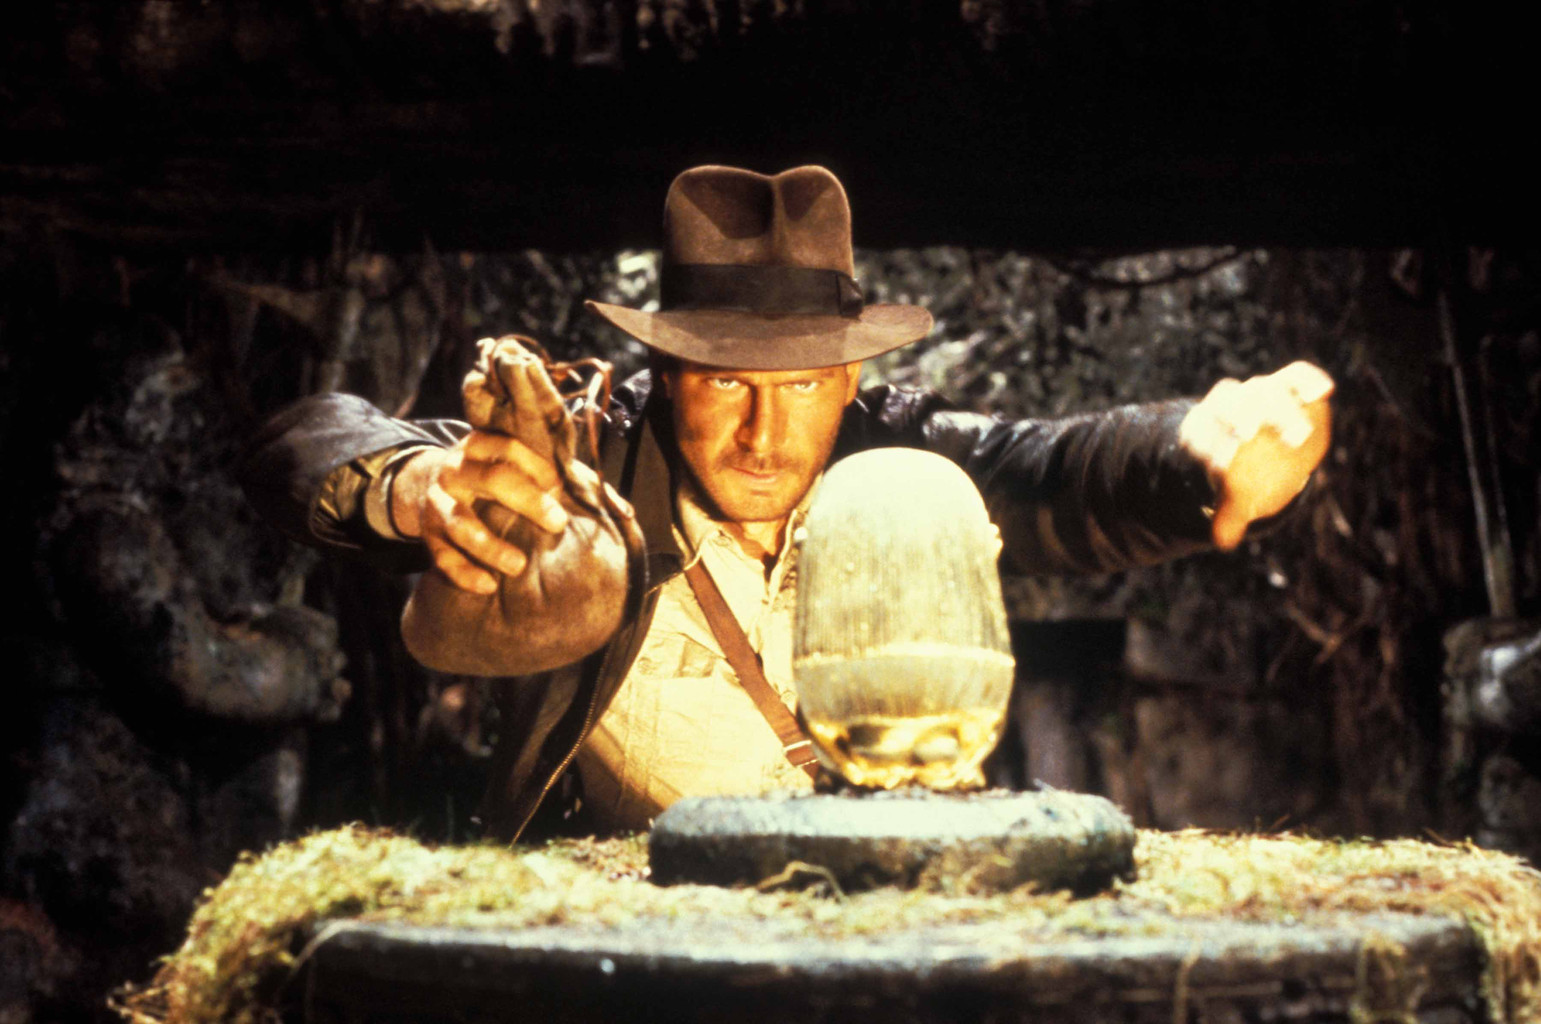
\includegraphics[width=\linewidth]{./media/images/indie}
  \tiny{\textit{Interactive Fiction readers are `doers' (Photo:
    \href{https://www.paramount.com/}{\textsc{paramount pictures)}}}}
}
%The \emph{Discoverer's Digest's} charter is to further the tradition of wonder through interactive play. The work strives to inspire new authors and readers. It hopes to spark new ideas on the shoulders of giants like Graham Nelson, Andrew Plotkin, Emily Short, Scott Adams, Bob Bates, Michael J. Roberts, and countless others. If this work touches an author to create solid experiences in ways never before seen then I personally consider this publication a success.

A high percentage of interactive fiction readers are also interactive fiction
writers. I like to think that those who read interactive fiction are `doers' by
virtue of their preference for taking an active role in their reading. You
authors are kindred souls, like the \emph{Indiana Jones'} of the literary world.
For this reason, \emph{Discoverer's Digest} is heavy on authorship content.
Topics ranging from using physical \textsc{gps} coordinates in your games to creating art that rivals commercial works even if you can't draw are covered.

Technical embelishment of the technical discussions in this issue lean primarily toward
\href{http://www.tads.org/tads3.htm}{\textsc{tads3}} on Linux. However, the
applications/methods I cite are almost always directly applicable to other,
similar applications using various operating systems.

\subsection{experience is everything}
\label{sec:experience_everything}
\marginnote{
  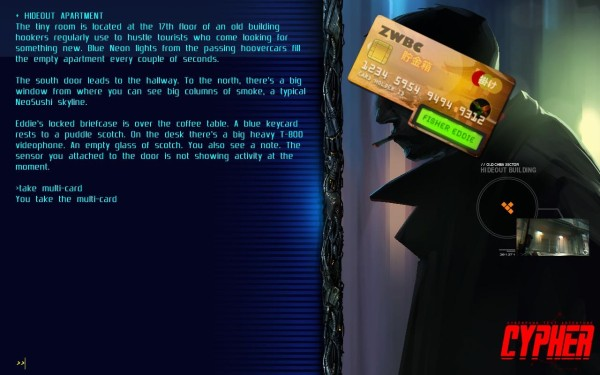
\includegraphics[width=\linewidth]{./media/images/cypher}
  \tiny{\textit{Cypher, an example work of modern interactive fiction (Photo: \href{gameenthusiest.net}{\textsc{gameenthusiest.net}})}}
}
The heart of Interactive Fiction is the medium's hold on people\ldots the way it
washes away your surroundings and transports you to another time and place. I
hope most of all to give the gift of a good story to all.

I give you in this issue a review of some ``old school'' \textsc{if} concepts
tied to modern, practical methods you can use to achieve an experience envisioned by the inspired authors in the past who found themselves
limited by the technology available at the time. My hope is that by using some
or all of the techniques outlined here that you truly immerse your
audience in your story and that they are better for it. 

All in all, I hope you enjoy this magazine. If you like, please feel free to submit your news,
story ideas, questions, and comments. \textit{Discoverer's Digest} seeks to
cover all manner of topics related to \textsc{if}, ranging from parser
experiences to choice\textemdash games, to experiments in the medium (including
General Artificial Intelligence) that we've not yet seen. This is especially true as
\href{https://ifcomp.org/}{\textsc{ifcomp}} is coming up and I'm excited about
that.

To submit you can simply send a personal email to

\href{mailto:cooper@cooper.stevenson.name}{\textsc{cooper@cooper.stevenson.name}}. \\ \\

\noindent Happy Writing! \\ \\

\noindent \href{mailto:cooper@cooper.stevenson.name}{\textsc{D. Cooper Stevenson}}

